\documentclass[hyperref={pdfpagelabels=false}]{beamer}
\usepackage{lmodern}
\usetheme{CambridgeUS}

\usepackage[english,brazilian]{babel}
\usepackage{multicol}
\usepackage{textcomp}
\usepackage[alf]{abntex2cite}
\usepackage[utf8]{inputenc}
\usepackage[T1]{fontenc}

\usepackage{amsmath,amssymb,exscale}

\title{Probabilidade e Estatística}  
\author[Matheus Pimenta]{Matheus Pimenta} 
\institute[UTFPR-CP]{\normalsize Universidade Tecnológica Federal do Paraná \\
	Câmpus Cornélio Procópio
} 
\date{ADNP 2020} 
\begin{document}
	
\begin{frame}
\titlepage
\end{frame} 


%\begin{frame}
%\frametitle{Table of contents}
%\tableofcontents
%\end{frame} 


\section{Erros de Decisão} 

\begin{frame}
\frametitle{Erros de Decisão}
Podemos cometer um erro de decisão quando feito o teste de hipótese: \pause
\begin{enumerate}
	\item Rejeitamos uma hipótese nula verdadeira: é o erro do tipo $I$; \pause
	\item Não rejeitamos uma hipótese nula falsa: é o erro do tipo $II$. \pause
\end{enumerate}

Resumidamente, se: \pause
\begin{itemize}
	\item $H_0$ é verdadeira, e rejeitamos, cometemos o erro do tipo $I$; \pause
	\item $H_0$ é falsa, e não rejeitamos, cometemos o erro do tipo $II$.
\end{itemize}
\end{frame}

\begin{frame}{Probabilidade de se cometer o erro do tipo $I$: $P(I)$}
Considere apenas testes bilaterais para o parâmetro $\mu$ da população normal com variância conhecida, isto é: \pause

$$\begin{cases}
H_0: \mu = \mu_0\\
H_1: \mu \neq \mu_0
\end{cases}$$

\end{frame}

\begin{frame}{Probabilidade de se cometer o erro do tipo $I$: $P(I)$}

Cometemos um erro do tipo $I$ quando rejeitamos $H_0$, ou seja, quando a amostra coletada possui uma média $\bar{x}$ que esta fora da região crítica (RC) do teste, isto é:
$$\bar{x} \in (-\infty,\bar{x}_1]\cup [\bar{x}_2,+\infty)$$ \pause

Dessa maneira, se $\mu_0$ é verdadeiro, então a probabilidade de cometer o erro do tipo $I$ é dada por:
$$P(I) = P(\bar{x} \in RC) = \alpha$$
$$P(I) = \alpha$$

\end{frame}

\begin{frame}{Probabilidade de se cometer o erro do tipo $I$: $P(I)$}
\begin{figure}
	\centering
	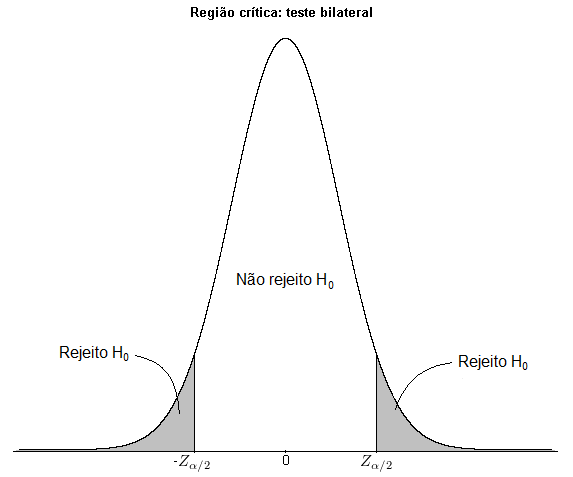
\includegraphics[width=0.7\linewidth]{teste}
	\label{fig:teste}
\end{figure}
\end{frame}

\begin{frame}{Probabilidade de se cometer o erro do tipo $II$: $P(II) = \beta$}

Após ter feito o primeiro teste, não rejeita-se $H_0:\mu = \mu_0$ como verdadeiro. \pause Posteriormente verifica-se que $H_0$ é falsa. Dessa maneira cometemos um erro do tipo $II$. \pause Para determinar a probabilidade precisamos inicialmente especificarmos como $H_1:\mu = \mu_1$. \pause
A um nível $\alpha$ temos:

$$\begin{cases}
H_0: \mu = \mu_0 \text{ (falso) }\\
H_1: \mu = \mu_1 \text{ (verdadeiro) }
\end{cases}$$ \pause

Não rejeitaremos $H_0$ quando $\bar{x} \in (\bar{x}_1, \bar{x}_2)$.

Como $H_0$ é falsa e a verdadeira média é dada por $H_1$, a distribuição dada por $H_0$ é falsa, então tem-se:

\end{frame}

\begin{frame}{Probabilidade de se cometer o erro do tipo $II$: $P(II) = \beta$}
	\begin{figure}
		\centering
		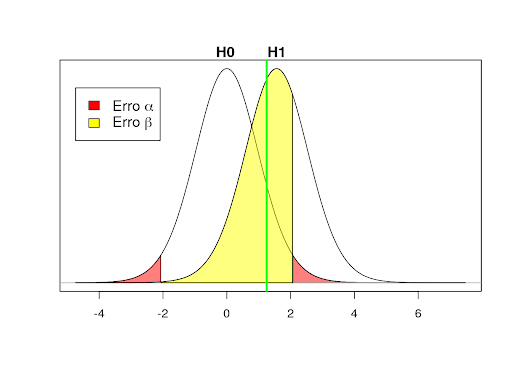
\includegraphics[width=0.9\linewidth]{erro2}
		\label{fig:teste2}
	\end{figure}
\end{frame}

\begin{frame}{Probabilidade de se cometer o erro do tipo $II$: $P(II) = \beta$}
Dessa maneira a probabilidade de cometermos um erro do tipo $II$ é a probabilidade de $\bar{x} \in (\bar{x}_1,\bar{x}_2)$, porém, com $\bar{x}$ se distribuindo com a média $\mu_1$, verdadeira: \pause


$$P(II) = \beta = P\{ \mu_0 - Z_{\alpha} \cdot \sigma_{\bar{x}} \leq \bar{x} \leq \mu_0 + Z_{\alpha} \cdot \sigma_{\bar{x}} | \mu_{\bar{x}} = \mu_1 \}$$
	
\end{frame}

\begin{frame}{Função Poder de um Teste ou Potência de um Teste}

A \emph{função poder de um teste} fornece a probabilidade de se rejeitar uma hipótese nula falsa. \pause

{\bf ATIVIDADE ASSÍNCRONA}
	
\end{frame}

\end{document}

